\documentclass{article}
% \usepackage[utf8]{inputenc}
\usepackage[english]{babel}
\usepackage[colorlinks]{hyperref}

\usepackage{float}
\usepackage{tocloft}
\usepackage{listings}
\usepackage{xcolor}
\usepackage{caption}
\usepackage{subcaption}
\usepackage{titlesec}
\usepackage{amsthm}
\newtheorem{prob}{Problem}
\usepackage[shortlabels]{enumitem}


\newtheorem{theorem}{Theorem}[section]
\newtheorem{corollary}{Corollary}[theorem]
\newtheorem{lemma}[theorem]{Lemma}

\definecolor[named]{myLayoutColorAux}{RGB}{174,49,54}
\definecolor[named]{myLayoutColorMain}{RGB}{0,26,153}
\definecolor[named]{myLayoutColorRed}{RGB}{255,0,0}
\usepackage{color}
\usepackage{menukeys}

\renewcommand{\cfttoctitlefont}{\color{myLayoutColorMain} \bfseries\Large}
\renewcommand{\cftloftitlefont}{\color{myLayoutColorMain} \bfseries\Large}



\titleformat*{\section}{\bfseries\Large\color{myLayoutColorMain}}

\begin{document}
\title{ECE275 Lab Final Project Kickoff}
\author{Vikas Dhiman}
\maketitle

\section{VGA module}

Watch the tutorial below and replicate it on the Altera FPGA board,

\begin{itemize}
\item
  VGA Video Tutorial (Must be logged in to you Umaine account to view) :
  \href{https://drive.google.com/file/d/1KwSqLo8CvzKBAjxMmDpdbc_UMAonZH9S/view?usp=sharing}{Video
  Tutorial}.
  There is a mistake in the video when instantiating the make box
  module, it should be make\_box make\_first\_player\_paddle( and not
  module make\_first\_player make\_box(
\item
  Example simple top level :
  \href{https://vikasdhiman.info/ECE275-Sequential-Logic/lab_pdfs/final_project_vga_files/VGA_top.v}{VGA\_top.v}
\item
  DE0 VGA Driver Module :
  \href{https://vikasdhiman.info/ECE275-Sequential-Logic/lab_pdfs/final_project_vga_files/DE0_VGA.v}{DE0\_VGA.v}
\item
  PLL (Phase Locked Loop) Verilog File :
  \href{https://vikasdhiman.info/ECE275-Sequential-Logic/lab_pdfs/final_project_vga_files/PLL_PIXEL_CLK.v}{PLL\_PIXEL\_CLK.v}
\item
  QSF File :
  \href{https://vikasdhiman.info/ECE275-Sequential-Logic/lab_pdfs/final_project_vga_files/VGA_top.qsf}{VGA\_top.qsf}
\end{itemize}



\section{Breaking application into smaller parts }
\subsection{Slow clock}

\begin{prob}
  A divide-by-N counter has one output and no inputs. The output Y is HIGH for
  one clock cycle out of every N. In other words, the output divides the frequency
  of the clock by N. The waveform for a divide-by-3 counter is shown here:\\
  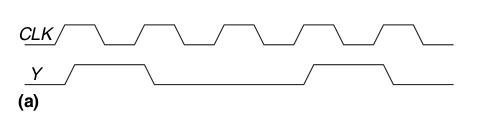
\includegraphics[width=0.8\linewidth]{./fig/fig.38a-divide-by-3-counter.png}\\
  Sketch circuit designs for such a counter
\end{prob}

\begin{prob}
  Repeat the above problem in Verilog and show a clock being reduced from 50 MHz
  to 10 Hz in ModelSim simulator. Example files covered in class,
  \href{https://vikasdhiman.info/ECE275-Sequential-Logic/lab_pdfs/pongproject-kickoff/slowclock/testslowclock.sv}{testslowclock.v}
    \href{https://vikasdhiman.info/ECE275-Sequential-Logic/lab_pdfs/pongproject-kickoff/slowclock/slowclock.sv}{slowclock.v}
\end{prob}


\subsection{Bouncing Ball}

\begin{prob}
  Design a circuit for a 1 pixel bouncing ball on a 4x4 pixel screen. You cannot design
this circuit by hand (Why?). How will you design it using Verilog? Write verilog
code and test it using a testbench?
\end{prob}

\begin{prob}
  Once you have the VGA example working, extend the above problem to 640x480
  resolution and ball represented by a box your chosen size. Connect this
  module's output to the VGA module.
\end{prob}

\subsection{Moving paddle}

\begin{prob}
 Design a circuit for 1 pixel paddle on a 4x4 pixel screen. Assume that it can
 take two inputs from BUTTONs, one for moving up and another one for moving
 down. You can design this circuit by hand (Why)?
\end{prob}

\begin{prob}
  Design the above circuit using Verilog.
\end{prob}

\begin{prob}
  Once you have the VGA example working, extend the above problem to 640x480
  resolution with you
\end{prob}

\subsection{Ball paddle collision}

\begin{prob}
  Combine the bouncing ball problem with the moving paddle problem and bounce
  the ball only if the ball is about to hit the paddle, otherwise game is over.
  If the ball hits the paddle increment a score counter by 1.
\end{prob}


\end{document}
